\clearpage
\setcounter{page}{1}
\maketitlesupplementary
\appendix

\section{Corpus details}
\label{sec:supp_data}

This section is the long form of \cref{sec:dataset}. Raw records, their calibration and orthorectification, and the selection of WAC and NAC records are shared with SomBench~\cite{patil2026sombench}; everything below the preprocessed products (the footprint grid, attachment of every layer, repeat observations on identical bounds, the sub-tile level, seam ownership, catalogs and splits) is specific to this corpus.

\begin{table*}[t]
  \centering
  \scriptsize
  \setlength{\tabcolsep}{3pt}
  \caption{All 34 layers of the corpus. Per-image products carry acquisition geometry and appear once per observation; static layers appear once per footprint. Polar layers exist only on the two polar caps. $r$: native resolution. Tile: pixels per side of a 60\,km footprint, $\lfloor 60\,\text{km}/r \rfloor$; for NAC and terrain, pixels per side of a 500\,m sub-tile. NaN\%: fraction of missing pixels, measured over every pixel of the released tiles (radar: reflectivity / CPR; WAC is zero by construction, since records with any missing pixel are rejected). Diviner bolometric temperature and GRAIL gravity are $4\times4$ and $3\times3$ rasters per footprint and are used only as coarse conditioning. Extent gives the latitude range of the source product.}
  \label{tab:layers}
  \resizebox{\textwidth}{!}{%
  \begin{tabular}{@{}llrrllrl@{}}
    \toprule
    Layer & Instrument / mission & $r$ (m) & Tile & Bands & Extent & NaN\% & Ref. \\
    \midrule
    \multicolumn{8}{@{}l}{\emph{Per-image (footprints)}} \\
    WAC visible & LRO LROC WAC & 100 & 600 & 415, 566, 604, 643, 689\,nm & global & 0.0 & \cite{robinson2010lunar,mahanti2016inflight} \\
    WAC ultraviolet & LRO LROC WAC & 500 & 120 & 321, 360\,nm & global & 0.0 & \cite{robinson2010lunar} \\
    \multicolumn{8}{@{}l}{\emph{Per-image (sub-tiles)}} \\
    NAC panchromatic & LRO LROC NAC & $\approx$1 & 500 & I/F & where imaged & 10.3 & \cite{robinson2010lunar,humm2016flight} \\
    NAC stereo terrain & LROC NAC DTMs & 3 & 166 & elevation, slope, aspect (sin, cos) & DTM sites & 5.0 & \cite{henriksen2017extracting} \\
    \midrule
    \multicolumn{8}{@{}l}{\emph{Static, equatorial and shared (16)}} \\
    Topography & SLDEM2015 (LOLA + Kaguya TC); LOLA polar & 60 & 1000 & elevation, slope, aspect (sin, cos) & global & 0.0 & \cite{barker2016new,barker2023new} \\
    Roughness & LOLA & 1000 & 60 & 50\,m-baseline roughness & global & 13.0 & \cite{kreslavsky2013lunar,neumann2015copernican} \\
    Morphologic mosaic & LROC WAC (643\,nm, high incidence) & 100 & 600 & 1 & global & 0.0 & \cite{speyerer2011lunar,wagner2015new} \\
    643\,nm normalized mosaic & LROC WAC, empirical photometric model & 100 & 600 & 1 & global & 0.26 & \cite{boyd2012lunar} \\
    Normalized reflectance & LROC WAC & 500 & 120 & 321--689\,nm (7) & $60^\circ$S--$60^\circ$N & 13.2 & \cite{boyd2012lunar} \\
    TiO$_2$ & LROC WAC (321/415\,nm ratio) & 400 & 150 & wt\% & $70^\circ$S--$70^\circ$N & 4.7 & \cite{sato2017lunar} \\
    MI reflectance & Kaguya Multiband Imager & 60 & 1000 & 414--1548\,nm (8) & $55^\circ$S--$55^\circ$N & 10.6 & \cite{ohtake2008performance,lemelin2016global} \\
    MI mineralogy & Kaguya MI inversion & 60 & 1000 & CPX, OPX, olivine, plag., grain size, FeO, OMAT & $50^\circ$S--$50^\circ$N & 23.4 & \cite{lemelin2015lunar,lemelin2016global} \\
    MI space weathering & Kaguya MI radiative transfer & 1000 & 60 & smFe, mpFe, npFe & $55^\circ$S--$55^\circ$N & 14.3 & \cite{trang2019improved} \\
    Rock abundance & LRO Diviner & 240 & 250 & areal fraction & $70^\circ$S--$70^\circ$N & 5.1 & \cite{powell2023high} \\
    Regolith temperature anomaly & LRO Diviner & 240 & 250 & K & $70^\circ$S--$70^\circ$N & 5.1 & \cite{powell2023high} \\
    H-parameter & LRO Diviner & 240 & 250 & m & $70^\circ$S--$70^\circ$N & 5.5 & \cite{hayne2017global} \\
    Radar & LRO Mini-RF (S-band) & 90 & 666 & S1 reflectivity, CPR & global & 42.5 / 43.5 & \cite{nozette2010lunar,fassett2024improved} \\
    Geologic map & USGS unified map & 60 & 1000 & 43 units (categorical) & global & 0.0 & \cite{fortezzo2020release} \\
    Bolometric temperature & LRO Diviner & 15000 & 4 & 24 local-time bins & global & 0.0 & \cite{williams2017global} \\
    Free-air gravity & GRAIL & 20000 & 3 & mGal & global & 0.0 & \cite{zuber2013gravity} \\
    \midrule
    \multicolumn{8}{@{}l}{\emph{Static, polar (14)}} \\
    Summer / winter temperature & LRO Diviner & 240 & 250 & 24 bins each (2 layers) & $80$--$90^\circ$ & $\approx$3 & \cite{williams2019seasonal} \\
    Ice stability depth & LRO Diviner + thermal model & 240 & 250 & m & $80$--$90^\circ$ & 27.4 & \cite{schorghofer2020mapping} \\
    Average illumination & LOLA DEM horizon model & 120 & 500 & fraction & $75$--$90^\circ$ & 0.0 & \cite{mazarico2011illumination} \\
    Permanently shadowed regions & LOLA DEM & 20 & 3000 & mask & $80$--$90^\circ$ & 0.0 & \cite{mazarico2011illumination,barker2023new} \\
    1064\,nm normal albedo & LOLA & 1000 & 60 & 1 & $50$--$90^\circ$ & 0.0 & \cite{lemelin2016improved} \\
    SP mineralogy & Kaguya Spectral Profiler & 1000 & 60 & olivine, plag., HCP, LCP, npFe, FeO, OMAT (7 layers) & $80$--$90^\circ$ & 4.3 & \cite{lemelin2022compositional} \\
    Hydrogen abundance & Lunar Prospector NS & 15000 & 4 & ppm & $60$--$90^\circ$ & 0.0 & \cite{lawrence2022global} \\
    \bottomrule
  \end{tabular}}
\end{table*}

\paragraph{Layers.} \Cref{tab:layers} lists the 34 layers: four per-image products (WAC visible and ultraviolet on the footprints, NAC panchromatic and NAC stereo terrain on the sub-tiles) and 30 static layers. Sixteen static layers cover the equatorial strips, and those whose source reaches the poles are also extracted on the caps; fourteen exist only on the caps. Static layers are present on 10,525 equatorial and 104 polar footprints. Every per-image record keeps the geometry of its acquisition (incidence, emission and phase angles, sub-solar ground azimuth, sub-solar and sub-spacecraft latitude and longitude, north azimuth), which conditions the predictor when the record is a target. Diviner bolometric temperature and GRAIL gravity hold only $4\times4$ and $3\times3$ pixels per footprint; they serve only as coarse conditioning and are not among the products of \cref{tab:modalities}. Any other layer can act as source or target.

\paragraph{Regions and projections.} Equatorial footprints live in one of 90 Lunar Transverse Mercator strips~\cite{mcclernan2025lunar}, 45 zones of $8^\circ$ longitude per hemisphere covering $|\phi| \le 82^\circ$; polar footprints live in a north or south polar stereographic cap covering $|\phi| \ge 82^\circ$. A footprint is a $3\times3$ block of GRAIL pixels, $60\times60$\,km in the projection of its region, and footprints are laid with a stride equal to their size. The footprint size must be an integer multiple of the 20\,km GRAIL pixel, so the master grid is never resampled. We use no overlap: two overlapping footprints would store pixel-identical static content over their intersection, the same WAC record would be clipped twice with the same acquisition geometry, so diversity sampling could not turn the duplicate into a new view, and each sub-tile under $m$ parents would be materialized $m$ times. Zones 1 and 45 are inset by $0.5^\circ$ from $\pm180^\circ$ to avoid warp artifacts of the virtual rasters at the discontinuity, footprints whose four-corner envelope spans more than $180^\circ$ of longitude are skipped, and whole zones can be excluded by configuration (off by default). Spatial matching of camera records to footprints is done in lunar geographic coordinates (IAU\_2015:30100) for the strips, where a footprint is a faithful box and the same index serves every strip. On the caps matching is done in projected coordinates, because a 60\,km square near the pole unprojects to a longitude range of hundreds of degrees, which no single swath can contain; records whose footprints become invalid or empty under projection to the cap, typically those from the opposite pole, are dropped when the index is built. A projection-compatibility checker rejects impossible source and target pairs, such as a polar stereographic record against a strip footprint, before any pixel is read.

\paragraph{Static-map extraction.} For each strip or cap, the GRAIL virtual raster cropped to the region defines the footprint centers and bounds, and every static layer is then read lazily from the region's virtual raster, which already holds it in the footprint's projection. Each layer is clipped to the footprint bounds at its native pixels, giving $t = \lfloor 60\,\text{km}/r \rfloor$ pixels per side (\cref{tab:layers}), from 1000 for SLDEM2015 to 3 for GRAIL; there is no reprojection and no snapping of the resolution at this stage. Layers whose source pixels do not align with the footprint origin, GRAIL and Diviner bolometric temperature, are resampled within the same projection to restore the exact $t\times t$ shape. Bands are stacked with their names, so a multi-band layer such as the eight MI reflectance bands stays addressable by wavelength. Each static layer is extracted once per footprint and shared by all WAC observations of that footprint and all NAC and terrain tiles of its sub-tiles. The image-anchored layout of SomBench instead re-clips every static layer for every image tile, which takes 21.5\,M netCDF files and 42.5\,TB against 9.5\,TB here. The polar registry adds the polar-only layers and polar projections of the shared ones; both registries emit catalogs with the same columns.

\paragraph{Per-image extraction.} Camera records are orthorectified products of~\cite{patil2026sombench}, each projected into the strip, or cap, that holds the largest fraction of its area, so a record can extend into neighboring strips. The WAC candidates of a footprint are the records whose geodatabase footprint polygons contain it, with incidence, emission and phase in $[0, 90]^\circ$ and sub-solar ground azimuth in $[0, 360]^\circ$; the pool holds 59,503 WAC products on disk. Extraction follows three rules. (i) Matching is done in geographic coordinates, or in projected ones on the caps (\cref{sec:grid}). (ii) A record whose strip equals the footprint's strip is sliced directly; otherwise the clip is cut in the record's own projection and only the clip is reprojected. The four footprint corners are transformed into the record's projection, the clip is enlarged by a 2-pixel buffer without resampling, reprojected to the footprint's projection and trimmed symmetrically, so no boundary pixel comes from edge padding. (iii) Every box transformed between projections uses the envelope of all four transformed corners, since the two-corner $(\min, \max)$ shortcut can swap the ordering of $x$ or $y$ under a nonlinear projection and silently truncate the footprint.

Two samplers select at most $k{=}500$ records per footprint. The default diversity-binned sampler places candidates on a two-dimensional illumination grid of 20 uniform incidence bins and $\operatorname{round}(k/20){=}25$ uniform sub-solar ground azimuth bins, with bin edges computed once per strip from the observed metadata range. Candidates are ordered by a randomized round-robin over occupied cells and extracted under a budget of five attempts per retained slot; the final selection again round-robins over cells, taking the lowest-NaN candidate within each cell first, so the kept set spans the available suns instead of collapsing onto the $k$ best-covered records, which are often near-duplicates. A record with any missing visible or ultraviolet pixel is rejected and the sampler continues down its ordering. Retained records are stored sorted by NaN fraction, so rank 0 is the best-covered observation. The alternative coverage-ranked sampler orders candidates by a 5:2 weighted mean of visible and ultraviolet NaN fraction and keeps the $k$ best, stopping early once $k$ complete records are found. Visible tiles have shape $(5, 600, 600)$ at 100\,m and ultraviolet tiles $(2, 120, 120)$ at 500\,m, and each record keeps its acquisition geometry, its rank and its combined NaN percentage. The result is 476,635 WAC records over 10,629 footprints; 9,232 footprints (86.9\%) have at least one, with 51.6 records per covered footprint on average (\cref{fig:illum}). This stack of co-registered images of the same ground under different suns is the supervision \method relies on.

\begin{figure}[t]
  \centering
  \begin{subfigure}[t]{0.49\linewidth}
    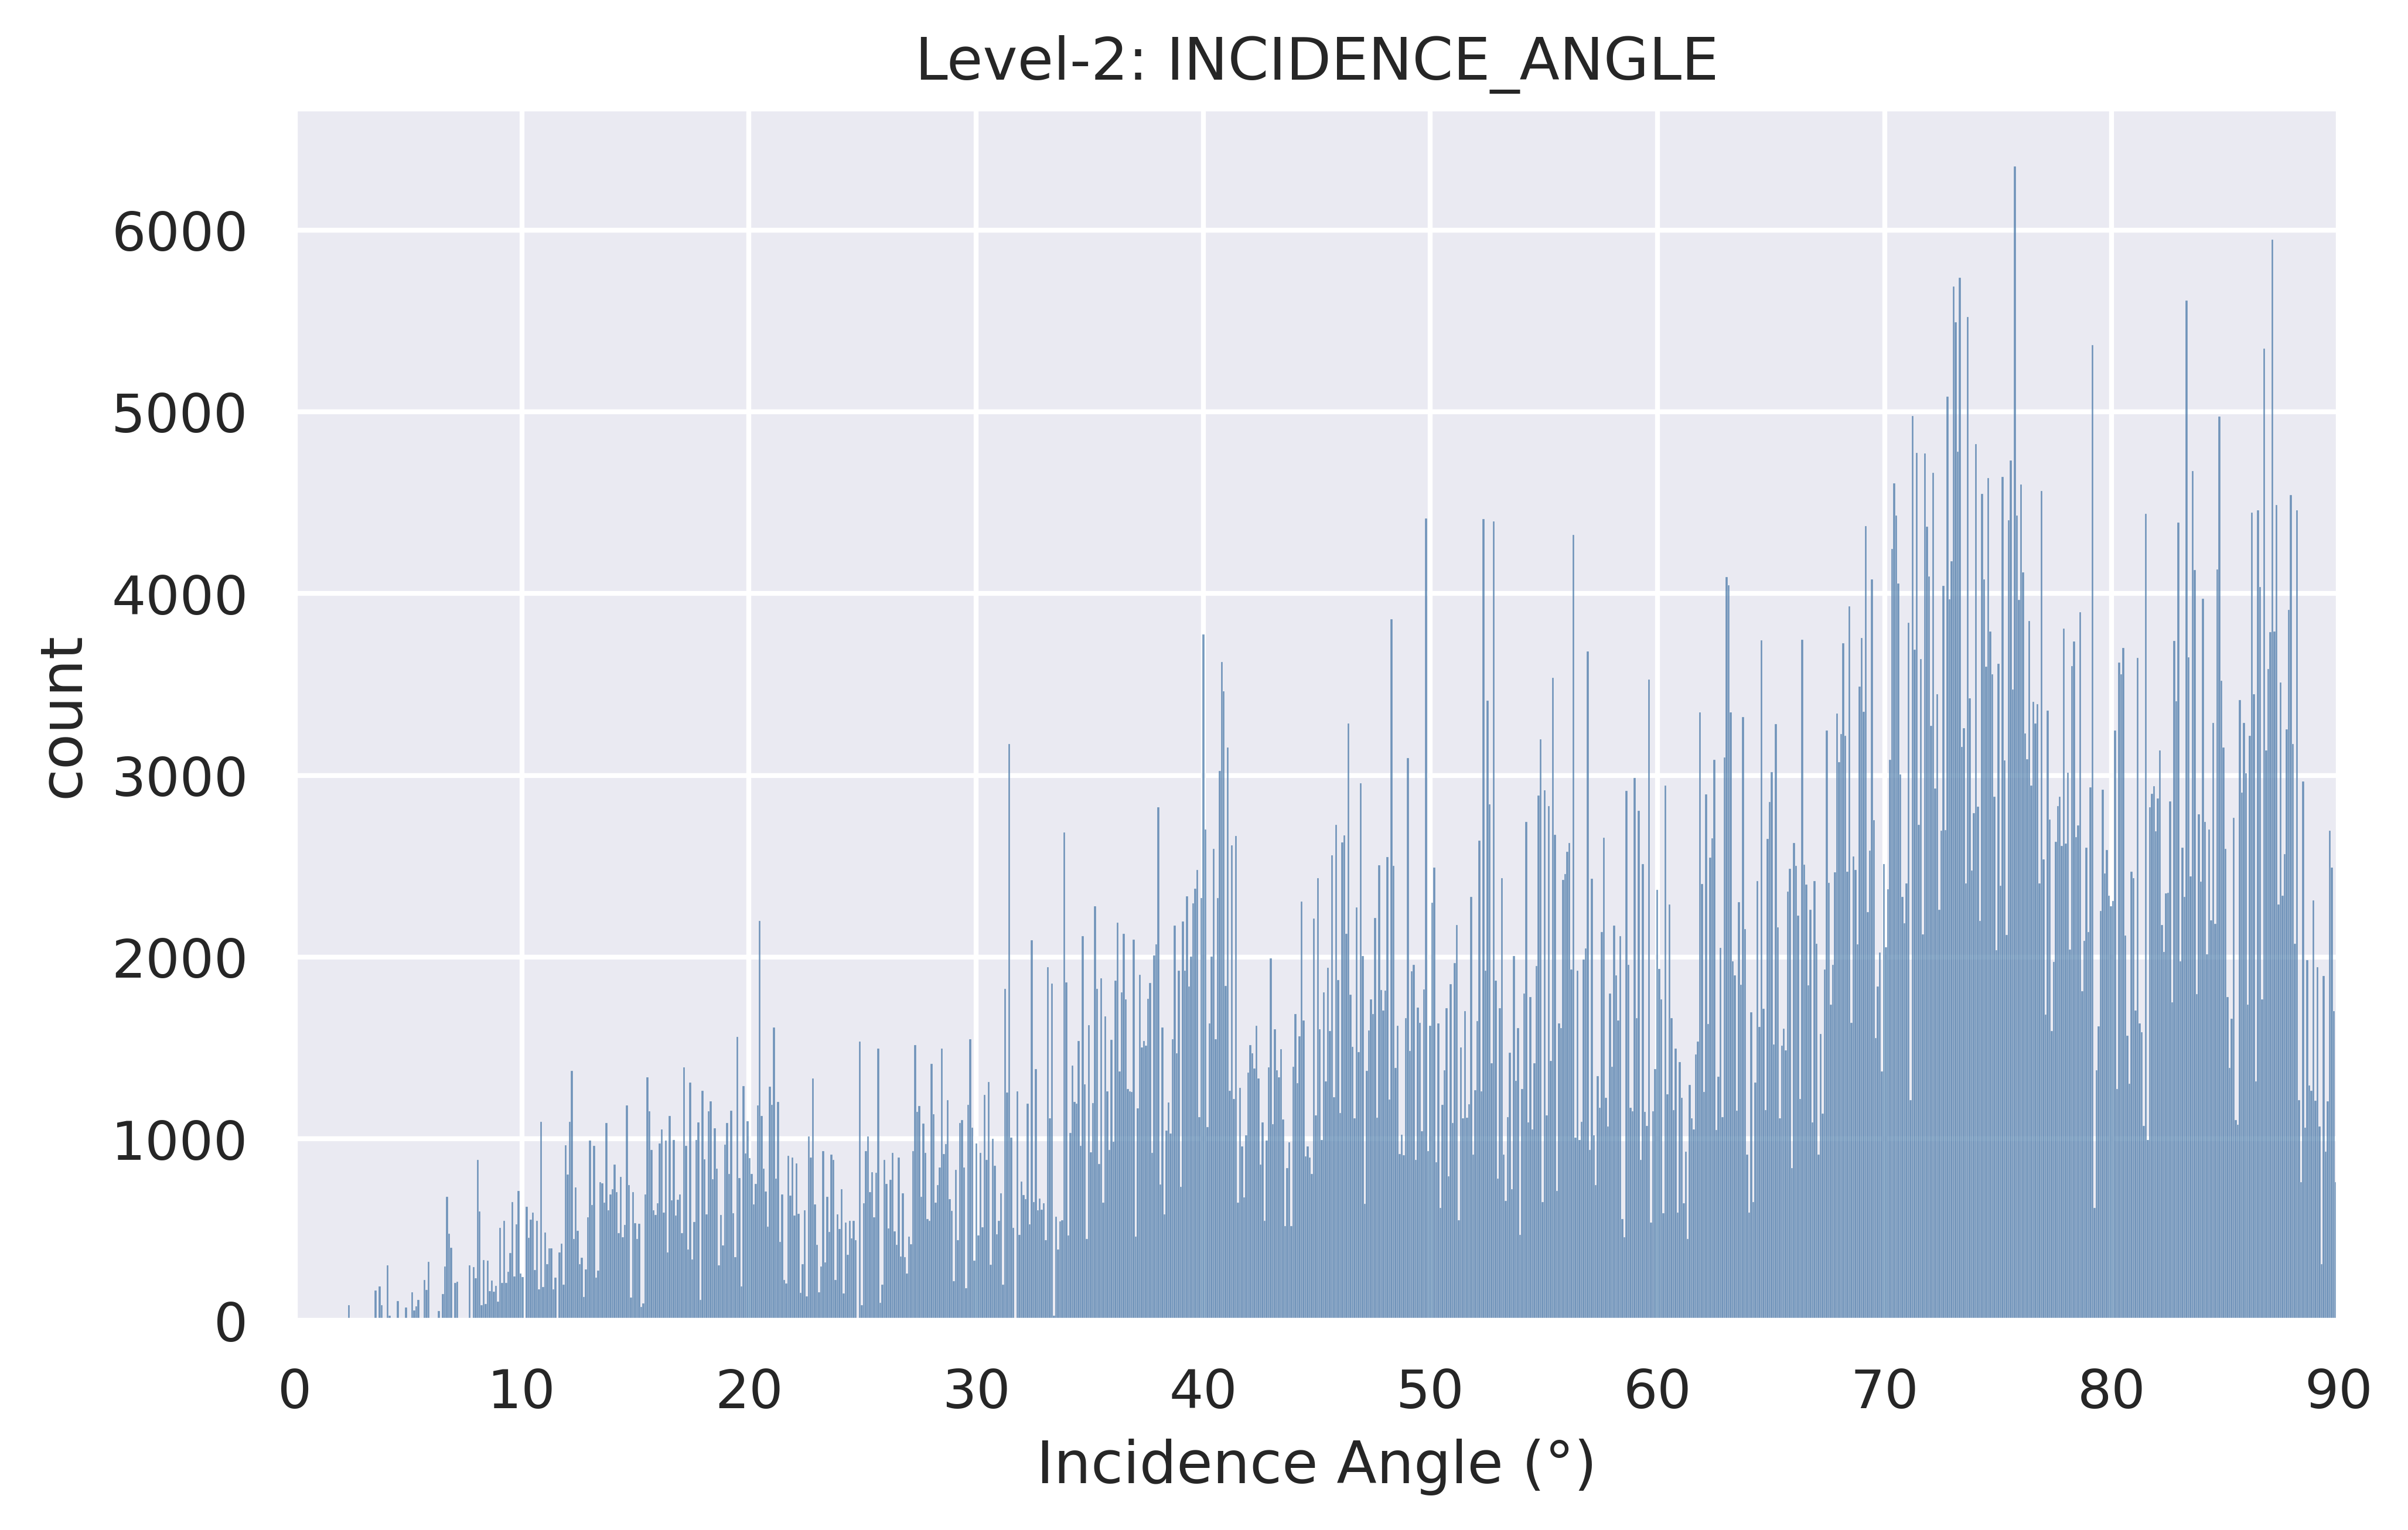
\includegraphics[width=\linewidth]{figures/level2_INCIDENCE_ANGLE.png}
    \caption{Incidence angle.}
  \end{subfigure}\hfill
  \begin{subfigure}[t]{0.49\linewidth}
    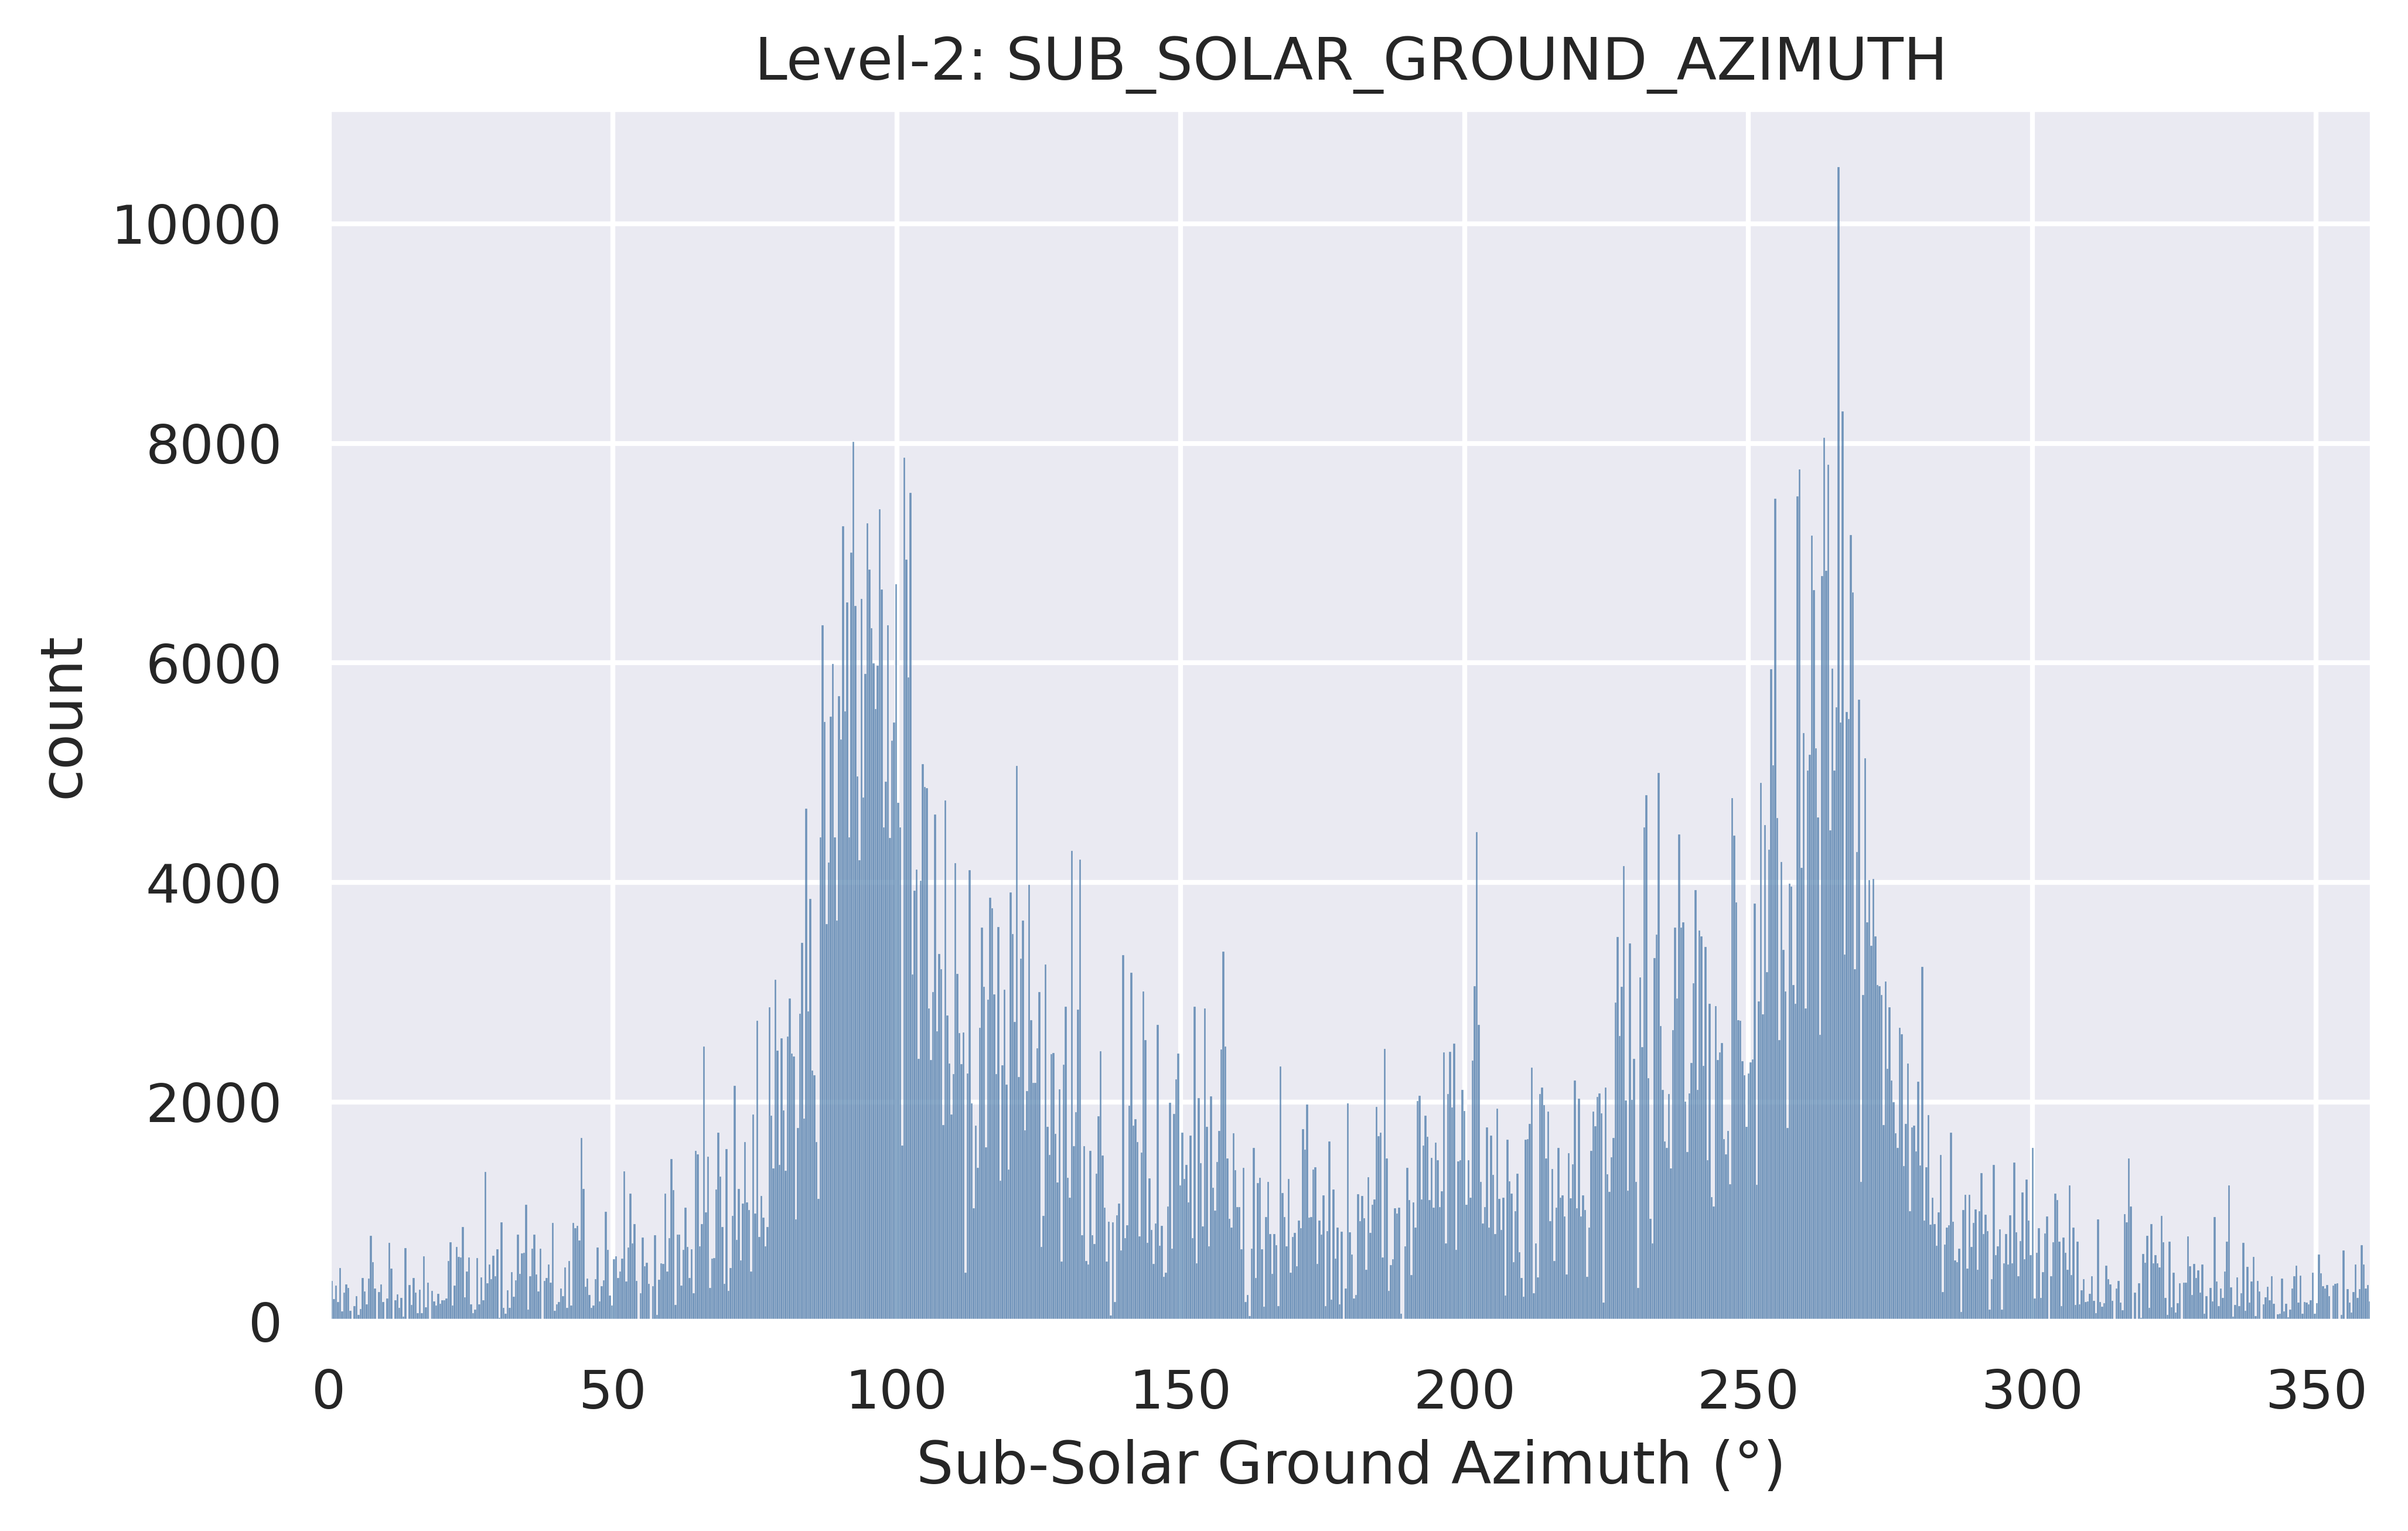
\includegraphics[width=\linewidth]{figures/level2_SUB_SOLAR_GROUND_AZIMUTH.png}
    \caption{Sub-solar ground azimuth.}
  \end{subfigure}
  \caption{Illumination of the NAC records retained over all 500\,m sub-tiles. The same diversity-binned sampler as for WAC bins each sub-tile's candidates on 20 incidence and 25 azimuth bins and fills the cells round-robin, lowest NaN first, up to $k{=}500$. The retained records spread over incidence up to $90^\circ$; the two azimuth peaks are inherited from the pool, since the sampler can only redistribute the geometries that a sub-tile's candidates offer.}
  \label{fig:illum_nac}
\end{figure}

\paragraph{Level 2.} NAC at about 1\,m on a 60\,km footprint would be 60,000 pixels per side ($3.6\times10^9$ cells per band), stereo terrain at 3\,m 20,000, and a NAC swath covers only a fraction of a footprint, so a footprint-sized canvas would be mostly missing. Each footprint is therefore divided into $120\times120$ sub-tiles of 500\,m (14,400 per parent) by the same grid generator, with geographic bounds from the four-corner envelope, an identifier that is a deterministic function of the sub-tile centroid and the parent, and a parent key. This step writes geometry and scalars only. A vectorized spatial join against the NAC and terrain footprint indexes drops sub-tiles with no candidate record and keeps per-source candidate flags; after extraction, sub-tiles with neither NAC nor terrain are pruned. Every static band of the parent is read once through a windowed, average-resampled read and reduced to a per-sub-tile mean (41 bands in the equatorial registry, 71 in the polar one; for maps coarser than the sub-tile this is the covering pixel), so a sub-tile carries its parent's state as scalars without a join.

NAC records are selected with the same diversity-binned sampler and $k{=}500$, ranked by NaN fraction (\cref{fig:illum_nac}). A record that covers only part of a sub-tile is placed at its true geographic offset in a $500\times500$ canvas filled with NaN, and canvases more than 99\% missing are never written; NAC tiles have shape $(1, 500, 500)$. Opening every matched record for every sub-tile would take about $5\times10^8$ clip-and-reproject operations. Extraction is instead batched by parent: each matched record is opened once per parent, a first pass computes the valid-pixel count of every sub-tile from an integral image of the reprojected record without materializing any canvas, the top-$k$ selection is made from these counts, and a second pass materializes only the selected (sub-tile, record) pairs. Reprojected arrays are processed in memory-bounded chunks, falling back to row strips for large records, and per-parent checkpoints make a strip resumable. Stereo terrain has five bands (elevation, slope, aspect and its sine and cosine); each sub-tile keeps the single record with the lowest elevation NaN fraction, under the same 99\% gate evaluated on elevation, as a $(5, 166, 166)$ tile. Eight equatorial strips intersect no terrain model at all (LTM 2N, 9N, 12N, 40N, 16S, 24S, 33S and 37S). The sub-tile level holds 5,354,773 sub-tiles with NAC or terrain, 9,453,706 NAC records after the exclusion of defective products (9,455,461 before), and 856,535 terrain records; 86.6\% of sub-tiles have NAC and 16.0\% terrain.

\paragraph{Catalogs and storage.} Each strip writes five Parquet catalogs (footprints, sub-tiles, and WAC, NAC and terrain records) and one directory per footprint holding one netCDF file per static layer and the footprint's WAC, NAC and terrain tiles. The catalogs share one column schema: identifiers (footprint, strip or cap, hemisphere or pole, parent for sub-tiles), projected and geographic centers and bounds with grid indices, one relative-path column per layer with a per-layer NaN summary, and for WAC and NAC records the acquisition geometry with rank and combined NaN percentage; terrain records carry no rank, and sub-tile rows add the candidate flags and the per-band static means. After all strips finish, the per-strip catalogs are unioned into global ones, and three merged tables are joined on the footprint identifier: Level 1 with one row per footprint and WAC rank (static columns repeated), Level 2 with one row per sub-tile and NAC rank (terrain columns prefixed), and a paired index of the Level-2 rows that hold both NAC and terrain (1,653,060 rows, 16.2\% of the Level-2 merge, counted before the NAC exclusion). Each Level-2 row also carries illumination-series statistics over its sub-tile's NAC records (count, minimum and maximum incidence and sub-solar ground azimuth), so consumers can pair the same ground under different suns without scanning the record catalog. Each tile is one netCDF file with one named variable per band, pixel-center $x$ and $y$ coordinates, the projection as WKT, Bitshuffle and LZ4 compression and one chunk per variable, so every file is self-describing. The catalogs are the only interface the training code reads. The corpus takes 9.5\,TB compressed (\cref{tab:corpus}).

\paragraph{Value registry.} Each band has a physical range (slope $[0, 90]^\circ$, reflectance $[0, 1]$, TiO$_2$ $[0, 100]$\,wt\%, elevation $[-9500, 10800]$\,m, roughness $[0, 20]$, ice stability depth $[0, 1]$\,m), applied at a single point, the netCDF write path, so no other code needs to clip. Clipping preserves NaN as a data gap and copies an array only when one of its bands needs it. Plagioclase grain size, which takes the classes 17 and 200\,\textmu m, is snapped to its classes; aspect is wrapped into $[0, 360)^\circ$ and stored also as sine and cosine; the categorical geologic map is left out of the registry, so its unit indices pass unchanged. The registry matters more than it looks. A scan of all 360 source rasters and 5,994 per-strip virtual rasters found the sources clean apart from a TiO$_2$ map without a declared no-data value, and found that cubic resampling in the virtual rasters multiplied no-data sentinels into neighboring pixels in most continuous layers (FeO up to $2{,}810$\,wt\%, aspect $-90$ to $450^\circ$, roughness $-0.73$). The registry removes these values before any statistics are computed. Of 11,392 NAC source files, six calibrated products contain defective pixels (values to $-29{,}542$) and five orthoimages are stored as raw counts without scale metadata; all eleven are excluded, and the 1,755 tiles already cut from two of them were removed.

\paragraph{Seam ownership.} A region keeps a candidate footprint when the footprint center lies inside it, so edge footprints reach up to half a footprint into the neighbor. Because each strip is tiled on its own projected GRAIL raster and narrows poleward, edge footprints of neighboring regions can cover up to 94\% of the same ground. Along every seam (strip to strip, north to south at the equator, strip to cap at $82^\circ$, zone 45 to zone 1 at the antimeridian) both regions would otherwise tile the same ground, in a sawtooth that depends on latitude. The ownership rule keeps the candidate with the larger share of its area inside its own region, measured on the exact projected squares after a great-circle prefilter, with ties to the lower-ranked region (strips before caps, then the lower zone number, then north before south). Each strip job derives its neighbors' candidate grids from the neighbors' GRAIL rasters and reaches the same decision independently, so the 92 jobs stay parallel. A model of the $0$--$82^\circ$ band estimates that the center rule covers 94\% of the band with 5.9\% covered twice, and the ownership rule covers 82\% with no ground covered twice, about 18\% fewer footprints; full containment would keep 65\% and empty everything above about $70^\circ$. The verification stage audits every seam with exact projected geometry at the start of each run and flags the corpus if any two footprints share ground, and the splitter refuses to write splits that share ground. \TODO{refresh counts after the seam repair; \cref{tab:corpus} predates it}

\paragraph{Splits.} Splits are assigned by whole LTM strips to train, validation and an optional test split, so nearby footprints never straddle a split. Strips are accumulated greedily by row count rather than strip count until the requested fraction is reached, so dense strips do not skew the proportions. The sub-tile and paired catalogs inherit the assignment of their parents. Each polar cap is a single region and would go wholly to one split, so in wedge mode each cap is cut into eight longitude wedges of whole footprints, and footprints poleward of $88^\circ$, where the wedges converge, are pinned to train. An option stratifies by hemisphere, splitting the northern strips, the southern strips and each cap independently, and an explicit list of held-out strips can override the assignment. Because a record can extend across a strip boundary, the splitter audits product-level leakage, source records that contribute rows to more than one split, and can drop the affected validation rows. A JSON manifest next to the split files pins the seed, fractions, polar mode, leakage statistics and per-split strip lists. Since seam ownership, the splitter measures ground overlap between splits on the exact projected footprint squares rather than on longitude and latitude boxes, and refuses splits that share ground. Pretraining in this paper uses the non-polar Level-1 rows. \TODO{non-polar train and validation footprint counts}

\section{Receptive-field offset of strided conv stems}
\label{sec:supp_stem}

Consider one stage with stride $s$, kernel $k$ and padding $q$ on a one-dimensional input of length $sn$ (pixels $0,\dots,sn{-}1$). Output $o$ reads input pixels $so{-}q,\dots,so{-}q{+}k{-}1$, so its receptive field is centered at $so - q + (k{-}1)/2$. The cell that output $o$ stands for spans pixels $so,\dots,so{+}s{-}1$, with center $so + (s{-}1)/2$. The offset of one stage is therefore
\begin{equation}
  \delta_1 = \frac{k-1}{2} - q - \frac{s-1}{2}.
\end{equation}
With $k{=}3$ and $q{=}1$, $\delta_1 = -(s{-}1)/2$ input pixels. Stacking stages with strides $s_1, \dots, s_n$ and total stride $P = \prod_j s_j$ gives, in native pixels,
\begin{equation}
  \delta = -\sum_{j} \Big(\prod_{i<j} s_i\Big)\frac{s_j-1}{2} = -\frac{P-1}{2},
\end{equation}
because the sum telescopes. In units of one token cell ($P$ pixels) this is \cref{eq:shift}. With $k{=}s{+}2$ and $q{=}1$, $\delta_1{=}0$ for every $s$, the receptive field extends one pixel beyond the cell on each side, and the output length is unchanged. At $s{=}3$ the $3\times3$ kernel reads pixels $3o{-}1,\dots,3o{+}1$; pixel $3n{-}1$ is never read, and two such stages leave the last four of 576 columns of a WAC tile unused. Stride-2 stages read every pixel at either kernel size.

\begin{table}[h]
  \centering
  \small
  \caption{Measured token offset (fraction of a cell, negative is up-left) and unread border columns with kernel 3, for the conv stems at $G{=}64$.}
  \label{tab:supp_shift}
  \begin{tabular}{@{}lccc@{}}
    \toprule
    $p$ (strides) & kernel 3 & kernel $s{+}2$ & unread cols \\
    \midrule
    4 (2, 2)          & $-0.375$ & 0 & 0 \\
    9 (3, 3)          & $-0.444$ & 0 & 4 \\
    16 (2, 2, 2, 2)   & $-0.469$ & 0 & 0 \\
    \bottomrule
  \end{tabular}
\end{table}

\section{Regularizers and position codes}
\label{sec:supp_reg}

\paragraph{VICReg covariance.} Let $z_{b,i}$ be the tokens of $K$ tiles, $v_b$ the mean of tile $b$ and $\bar v$ the mean over tiles. The covariance over all tokens splits into a within-tile and a between-tile part,
\begin{equation}
  C = \frac{1}{KN}\sum_{b,i}(z_{b,i}-v_b)(z_{b,i}-v_b)^\top + \frac{1}{K}\sum_b (v_b-\bar v)(v_b-\bar v)^\top.
\end{equation}
For a position code, $z_{b,i} = u(i)$ in every tile, so $v_b = \bar v$ and the second term is zero. When tiles differ in content, the second term adds off-diagonal entries, and with few tiles per batch these can be large. For the same within-tile structure, the penalty is therefore lower for a position code.

\paragraph{Pooled SIGReg.} Let $t_1, \dots, t_N$ be the layer-normalized tokens of a tile, so that $\|t_i\|^2 = D$, and let $\bar m$ be their mean. Then $\|\bar m\|^2 = D\,\bar c$, where $\bar c$ is the mean cosine similarity between tokens of the tile. Matching $\mathcal{N}(0, I_D)$ requires $\E\|\bar m\|^2 = D$, so $\bar c \approx 1$, which means nearly identical tokens within each tile.

\paragraph{Variance hinge on predictions.} The best prediction under a squared-type loss is $\hat z = \E[\bar z \mid \text{source}]$. By the law of total variance, its variance per feature is $R^2$ times the target variance, where $R^2$ is the fraction of the target variance that the source explains. With layer-normalized targets the target variance is about one, so a hinge at a standard deviation of 1 can only be met by adding variance that the source does not explain.

\section{Runs}
\label{sec:supp_runs}

\Cref{tab:supp_runs} lists every run this paper cites. All runs use the ViT-B encoder with four MoE layers (except A3) and the 12-layer predictor, four supervision depths, $M{=}2$ targets, a single source and a visible block of 70--80\% (except B1 and B2, which see the full source). The variance hinge is on for evidence and predictions with $\gamma{=}1$ except in F4 and F5. SIGReg is off in every run listed. $\Delta$ and $S$ are validation values at the last step; max $S$ is taken after 5k steps.

\begin{table*}[t]
  \centering
  \scriptsize
  \setlength{\tabcolsep}{3pt}
  \caption{Runs cited in the paper. Stems: shared canvas (C) or fixed-GSD with kernel floor $k_{\min}$ (F$k$). EMA: constant 0.996 (c) or cosine ramp to 0.9995 (r). Batch: effective footprint rows per optimizer step. $^\ddagger$Seven products configured; the raster gate of the shared-canvas path drops LOLA roughness at $G{=}64$, leaving six.}
  \label{tab:supp_runs}
  \begin{tabular}{@{}llcccccccccccl@{}}
    \toprule
    ID & Run & $G$ & Prod. & Stems & $S_{\max}$ & LR & Batch & EMA & $w_c$ & Steps & $\Delta$ & $S$ & max $S$ / outcome \\
    \midrule
    A1 & MoE, $k_{\min}{=}1$                                 & 64  & 12 & F1 & 1000 & 3e-5 & 256  & r & 0.01  & 97.5k  & .167 & .16  & .56 / healthy \\
    A2 & MoE, $k_{\min}{=}4$                                 & 64  & 12 & F4 & 1000 & 3e-5 & 256  & r & 0.01  & 97.5k  & .121 & .25  & .42 / healthy \\
    A3 & dense, $k_{\min}{=}1$                               & 64  & 12 & F1 & 1000 & 3e-5 & 256  & r & 0.01  & 112.5k & .119 & .51  & .71 / healthy \\
    B1 & long-short attention                                & 64  & 12 & F1 & 600  & 3e-5 & 256  & r & 0.01  & 35k    & .000 & 1.00 & 1.00 / position code \\
    B2 & long-short + border clamp                           & 64  & 12 & F1 & 4096 & 3e-5 & 256  & r & 0.01  & 60k    & .000 & 1.00 & 1.00 / position code \\
    C1 & $w_c{=}0.005$                                       & 32  & 5  & C  & 600  & 1e-4 & 3072 & c & 0.005 & 9k     & .181 & .48  & .48 / rank falling, stopped \\
    C2 & $w_c{=}0.05$                                        & 32  & 5  & C  & 600  & 1e-4 & 3072 & c & 0.05  & 8.5k   & .003 & .91  & .91 / position code \\
    D1 & $S_{\max}{=}600$                                    & 64  & 7  & F1 & 600  & 1e-4 & 96   & c & 0.005 & 54k    & .069 & .81  & .81 / dimensional \\
    D2 & $S_{\max}{=}1000$                                   & 64  & 7  & F1 & 1000 & 1e-4 & 96   & c & 0.005 & 118k   & .120 & .66  & .90 / dimensional \\
    D3 & 50\% NAC rows                                       & 64  & 12 & F1 & 1000 & 1e-4 & 256  & c & 0.01  & 160k   & .024 & .97  & .99 / dimensional \\
    E1 & shared canvas, 5 prod.                              & 64  & 5  & C  & 1000 & 5e-5 & 128  & c & 0.01  & 65k    & .127 & .67  & .67 / dimensional, diverged \\
    E2 & fixed-GSD, 5 prod.                                  & 64  & 5  & F1 & 1000 & 5e-5 & 128  & c & 0.01  & 82.5k  & .060 & .38  & .69 / healthy \\
    F1 & grid sweep                                          & 32  & 12 & F4 & 4096 & 3e-5 & 256  & r & 0.01  & 10k    & .009 & .55  & .55 / short \\
    F2 & grid sweep                                          & 64  & 12 & F4 & 4096 & 3e-5 & 256  & r & 0.01  & 10k    & .010 & .77  & .77 / short \\
    F3 & grid sweep                                          & 128 & 12 & F4 & 4096 & 3e-5 & 256  & r & 0.01  & 10k    & .016 & .63  & .63 / short \\
    F4 & F2, no hinge on $\hat z$                            & 64  & 12 & F4 & 4096 & 3e-5 & 256  & r & 0.01  & 10k    & .055 & .24  & .24 / short \\
    F5 & F2, hinge $\gamma{=}0.3$ on $\hat z$                & 64  & 12 & F4 & 4096 & 3e-5 & 256  & r & 0.01  & 2.5k   & .033 & .30  & -- / stopped \\
    G1 & dense loss + conv stems                             & 32  & 7  & C  & 600  & 1e-4 & 768  & c & 0.005 & 40k    & .283 & .23  & .23 / healthy, running \\
    G2 & closest earlier run                                 & 32  & 7  & C  & 600  & 1e-4 & 768  & c & 0.005 & 48.5k  & .062 & .51  & .67 / healthy \\
    H  & downstream backbone                                 & 64  & 6$^\ddagger$ & C & 600 & 1e-4 & 512 & c & 0.005 & 79k & .046 & .57 & .74 / used downstream \\
    I  & within-tile smoothing                               & 64  & 12 & F1 & 1000 & 5e-5 & 128  & c & 0.01  & 87.5k  & .082 & .55  & .67 / smoothing \\
    \bottomrule
  \end{tabular}
\end{table*}

\paragraph{Shared recipe.} Unless stated otherwise: ViT-B encoder with the last four blocks MoE (8 experts, top-2), 12-layer predictor of width 768, four supervision depths, visible square block covering 70--80\% of the grid, $M{=}2$ targets per row, VICReg variance weight 1 on evidence and predictions, covariance 0.005--0.01, no SIGReg, EMA decay 0.996 (constant or ramped to 0.9995), AdamW with weight decay 0.05 and clipping at 1, warmup over 10\% of the schedule, cosine decay to $10^{-6}$.

\paragraph{Runs in \cref{tab:signals}.} The two long-short attention runs use $G{=}64$, fixed-GSD stems with $k_{\min}{=}1$, 12 products, no source masking, peak learning rate $3{\times}10^{-5}$ and $w_c{=}0.01$. The second adds the border clamp and uses $S_{\max}{=}4096$ instead of 600. The $w_c{=}0.05$ run uses $G{=}32$, shared-canvas stems, 5 products and peak learning rate $10^{-4}$ at an effective batch of 3072, and differs from its $w_c{=}0.005$ twin only in that weight. The twin is not a clean healthy reference: over its last 4k steps, before it stopped at 9.3k, its within-tile rank fell from 384 to 120 while its covariance rose from 5.7 to 14.8, the early signature of dimensional collapse, with $S$ at 0.38. The pair shows only that the larger weight produced a position code. The fixed-GSD pair uses $G{=}64$, seven products, $k_{\min}{=}1$ and peak learning rate $10^{-4}$, and differs only in $S_{\max}$. The 50\%-NAC run uses 12 products at $G{=}64$ and draws half of its rows from the 500\,m NAC sub-tiles. The shared-canvas run is the baseline arm of the five-product stem comparison of \cref{sec:exp_tokens}.

\paragraph{Collapse labels.} To evaluate monitors independently of themselves we fit two linear probes on frozen target tokens and score them on held-out footprints. A content probe predicts physical values of other products at each cell (elevation and slope from a WAC token, for example); a position probe predicts the cell coordinates. A checkpoint is labeled a position code when the content $R^2$ drops below 10\% of the run's maximum while the position $R^2$ stays above 0.9, and dimensionally collapsed when the effective rank of tile-mean embeddings drops below 10\% of the run's maximum.

\paragraph{Downstream backbone.} $G{=}64$, shared-canvas stems, products WAC visible, WAC UV, elevation, slope, aspect and the 643\,nm mosaic. LOLA roughness was configured but dropped by the raster-size gate of the shared-canvas path. $S_{\max}{=}600$, peak learning rate $10^{-4}$, constant EMA 0.996, $w_c{=}0.005$, effective batch 512, 79.1k steps, final $\Delta{=}0.046$ and $S{=}0.57$.

\section{Kernel floor per product pair}
\label{sec:supp_floor}

\Cref{tab:floor} breaks the kernel-floor comparison of \cref{sec:exp_tokens} (runs A1 and A2) down by groups of product pairs.

\begin{table}[t]
  \centering
  \footnotesize
  \setlength{\tabcolsep}{3.5pt}
  \caption{Kernel floor, per group of product pairs (validation $\Delta$ at 97.5k steps, macro average over pairs; 12 products, grid 64). The floor affects LOLA roughness (1 px/token at $k_{\min}{=}1$) and the 500\,m and 400\,m WAC products (2 px/token).}
  \label{tab:floor}
  \begin{tabular}{@{}lccc@{}}
    \toprule
    Pairs & \#pairs & $k_{\min}{=}1$ & $k_{\min}{=}4$ \\
    \midrule
    Roughness as target                & 11 & 0.033 & \textbf{0.103} \\
    Roughness as source                & 11 & 0.023 & \textbf{0.100} \\
    TiO$_2$ as target                  & 11 & 0.079 & \textbf{0.112} \\
    WAC UV as target                   & 11 & \textbf{0.145} & 0.134 \\
    Pairs without floored products     & 42 & \textbf{0.205} & 0.122 \\
    \midrule
    Overall (count-weighted)           & 132 & \textbf{0.167} & 0.121 \\
    \bottomrule
  \end{tabular}
\end{table}

\section{Downstream protocols}
\label{sec:supp_downstream}

\Cref{tab:safs} lists all relief, albedo and shadow probe metrics of \cref{sec:downstream}.

\begin{table}[h]
  \centering
  \footnotesize
  \setlength{\tabcolsep}{4pt}
  \caption{Relief, albedo and shadows from frozen features (40 held-out footprints, 8 suns each). Invariance: correlation between predictions for one footprint under different suns. Retrieval: top-1 accuracy of matching a prediction to its footprint.}
  \label{tab:safs}
  \begin{tabular}{@{}lc@{}}
    \toprule
    Probe and metric & Value \\
    \midrule
    \multicolumn{2}{@{}l}{\emph{WAC $\to$ relief, linear probe}} \\
    \quad correlation (same probe on pixels: 0.12) & 0.705 \\
    \quad sun invariance / retrieval               & 0.90 / 0.96 \\
    \multicolumn{2}{@{}l}{\emph{WAC $\to$ albedo, linear probe}} \\
    \quad correlation with the 643\,nm mosaic       & 0.840 \\
    \quad sun invariance / retrieval               & 0.87 / 1.00 \\
    \multicolumn{2}{@{}l}{\emph{WAC $\to$ relief, SAFS head}} \\
    \quad correlation / RMSE (zero relief: 551\,m)  & 0.808 / 299\,m \\
    \midrule
    \multicolumn{2}{@{}l}{\emph{DTM + sun $\to$ WAC shadows, linear probe}} \\
    \quad AUC with the true sun                     & \textbf{0.89} \\
    \quad AUC with another observation's sun        & 0.59 \\
    \quad AUC with no sun                           & 0.49 \\
    \bottomrule
  \end{tabular}
\end{table}

\paragraph{Crater detection.} Robbins 1k has 800/100/100 WAC tiles of 512\,px at 100\,m drawn from the test split of SomBench~\cite{patil2026sombench} with incidence between $60^\circ$ and $80^\circ$; Robbins 10k has 8000/1000/1000 tiles with a wider range of illumination; the NAC set has 289/63/56 hand-labeled tiles of 256\,px at 0.8--5\,m from six photometry sites, labeled with OpenCraterTool~\cite{heyer2023comparative}. The detectors read the frozen EMA encoder at its four supervision depths through a trainable three-level feature pyramid. The per-product stems are fine-tuned with the neck and head at learning rate $10^{-4}$, while the transformer stays frozen. We train with multi-scale native crops. The pixel branch is a shallow convolution on the raw input that feeds the finest pyramid level. Our protocol scores all boxes down to 2\,px with at most 300 detections. The NASA-IBM protocol keeps boxes with a shortest side of at least 10\,px, drops tiles without craters and allows 500 detections. In that protocol the NASA-IBM backbone is fully frozen, whereas our stems are fine-tuned, a difference in our favor. The predicted DTM comes from a DPT head trained on the backbone's elevation-product predictor features, given the WAC image.

\paragraph{Relief, albedo and shadows.} Footprints with at least six observations are split, with a fixed seed, into 120 for fitting and 40 for evaluation. Outputs are 128\,px (469\,m per pixel). The relief target is the plane-detrended 60\,m DTM. Albedo is scored against the 643\,nm mosaic and, separately, against a multi-sun pseudo-albedo. The linear probes read frozen predictor features. The relief head fuses the elevation-product features across depths, is conditioned on the sun, and integrates predicted slope and aspect with a Frankot--Chellappa solver; it was fitted on 600 footprints with two suns each. Shadow labels are the darkest-quantile pixels of the WAC image on high-incidence observations, where dark pixels are mostly cast shadow.

\paragraph{Irregular mare patches and ice prospectivity.} The segmentation benchmark has 100/20/10 NAC tiles of 256\,px at 1\,m with pixel masks~\cite{patil2026sombench,hargitai2025clusters}; the prospectivity benchmark regresses a 0--1 ice-prospectivity map from eight polar evidence layers at 240\,m on 108/24/25 patches~\cite{coyan2025prospectivity}. \TODO{protocols and results for both tasks}
